\section{Additional Optimizations}
\label{sec:opts}

Figure~\ref{fig:batching} shows the performance benefits of batching log
appends for two different implementations. The \emph{simple} implementation
uses internal I/O interfaces to process each append independently, and the
modest performance benefits are due to the amatorization of the fixed
per-request cost. The \emph{batch-aware} implementation is able to achieve much
higher performance by constructing more efficient I/O requests using range
queries and data sieving.

\begin{figure}
\centering
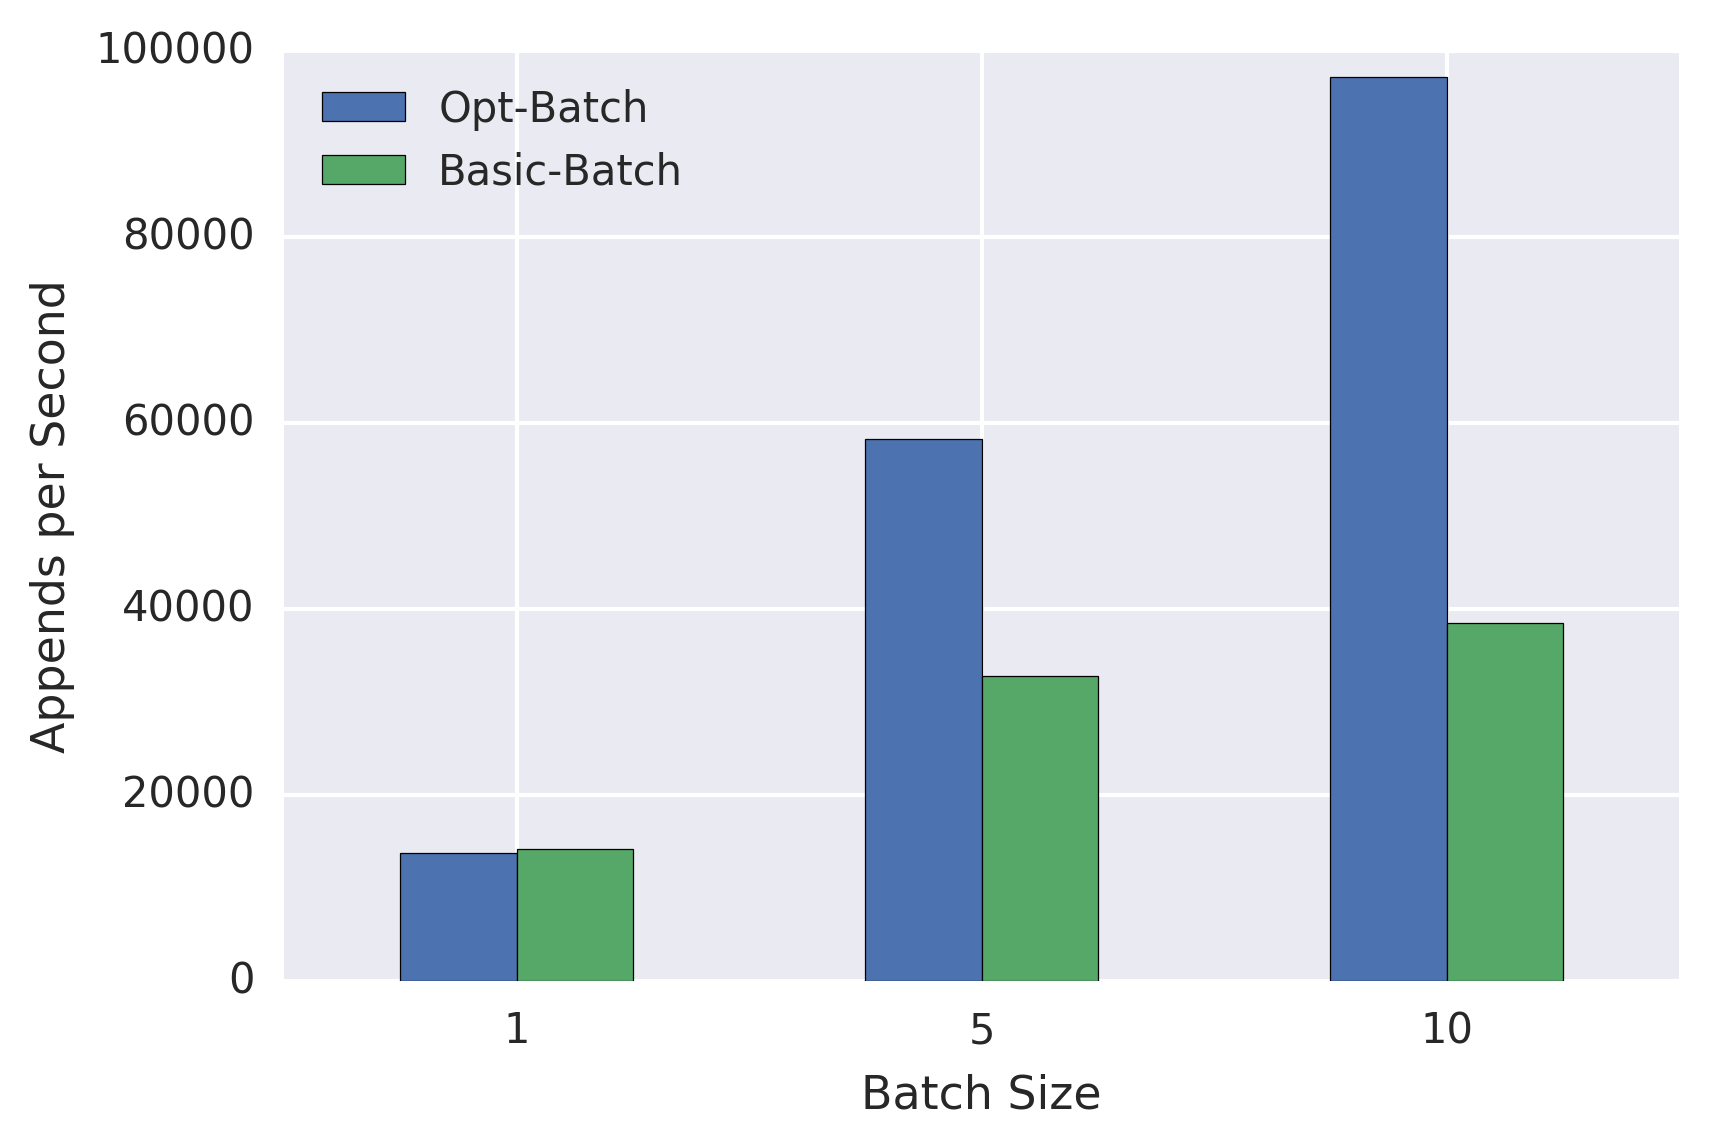
\includegraphics[width=1.0\linewidth]{batching.png}
\caption{Total throughput with and without batching.}
\label{fig:batching}
\end{figure}

While the performance impact of application-specific batching is significant,
techniques such as range queries and data sieving are sensitive to outliers.
For example, handling two requests independently will become more efficient
than using a data sieving technique as the size of the range between the
requests increases. Figure~\ref{fig:batching-outlier} highlights this
challenge. The \emph{simple} implementation has consistent, but relatively
worse performance. The \emph{batch-aware} implementation achieves high append
throughput, but performance degrades as the magnitude of the batch outlier
increases. In contrast, the \emph{batch-oident} applies a simple heuristic to
identify the outlier and handle it independently, resulting in only a slight
decrease in performance over the best case.

\begin{figure}
\centering
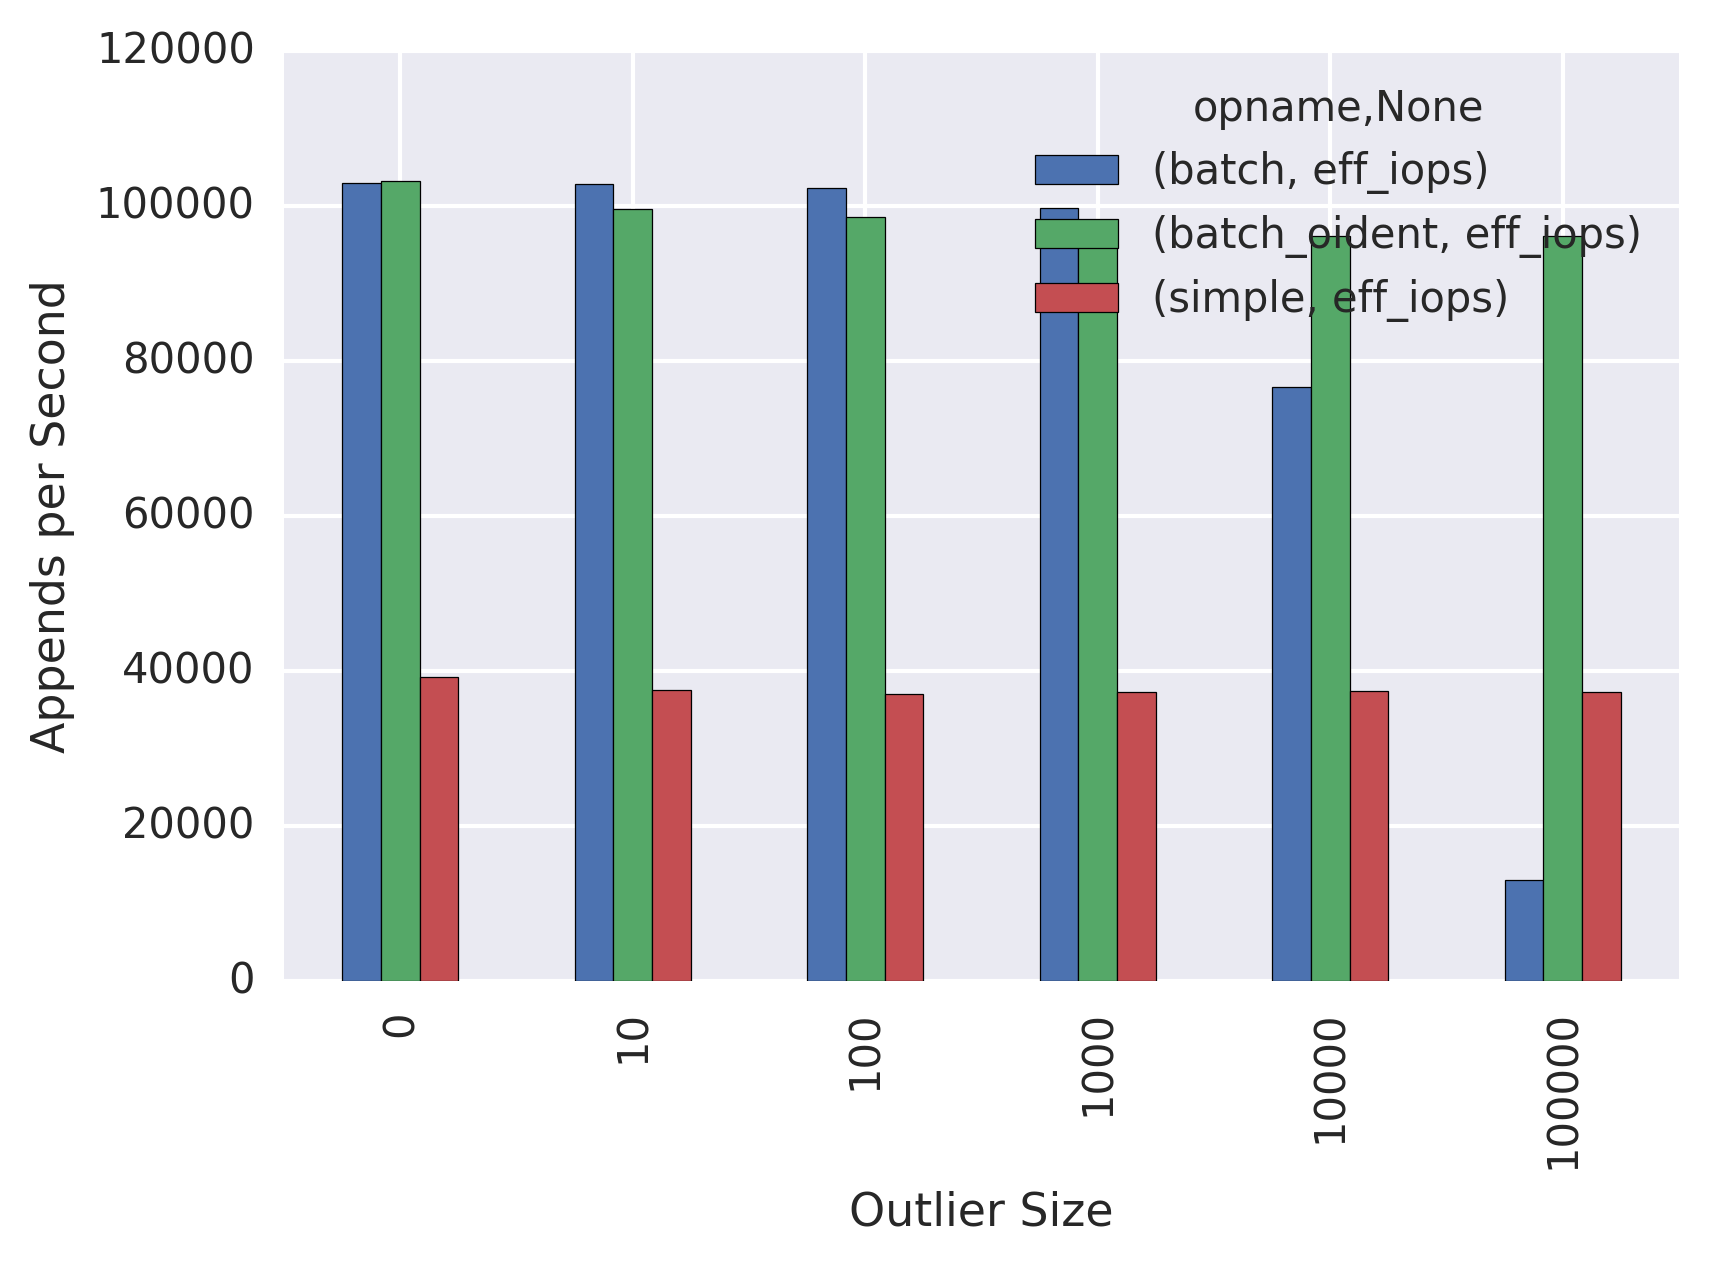
\includegraphics[width=1.0\linewidth]{batching-outlier-detect.png}
\caption{Identifying and handling an outlier independently maintains the
beneifts of batching without the performance degredation of unecessarily
large I/O requests.}
\label{fig:batching-outlier}
\end{figure}
